\subsection{If a parent class imports a class from different package, the target child class cannot be duplicate with that imported class after rename.}

If we try renaming a subclass with the same name as the class imported into its parent class from another package, compiler produces the error as `a compilation unit must not import and declare a type with the same name'~\cite{EclipseWebPage}. 
To rename a class or subclass for refactoring the code, some of the necessary preconditions have to be checked. This precondition can be explained by the following example.

\begin{figure}[th]
\centering
\begin{minipage}[t]{0.45\linewidth}
\begin{lstlisting}[language=java, basicstyle=\scriptsize\ttfamily,frame=single]	
package q;
import p.C;
class A{	
}
class B extends A{	
}	
\end{lstlisting}
\tiny{(a) Before renaming Subclass B}
\end{minipage}
\hfill
\begin{minipage}[t]{0.45\linewidth}
\begin{lstlisting}[language=java, basicstyle=\scriptsize\ttfamily,frame=single]
package q;
import p.C;
class A{	
}
class C extends A{	
}	
\end{lstlisting}
\tiny{(b) After Renaming Subclass B to C}
\end{minipage}
\caption{Precondition for Renaming Sub-class}
\label{figure:fig7}
\end{figure}

From the above figure \ref{figure:fig7}, We see that if one has imported class C from  package  p to the parent Class A and if we try to rename the sub-class B to C, Compiler produces  the error as given in the figure \ref{figure:fig8} . As mentioned in  section \ref{sec:precon2}, the same precondition also holds good for renaming a sub-class. Before renaming the sub-class, one has to check the precondition that the  target sub-class cannot be duplicate with any imported class into its parent class from another package.

\begin{figure}[htbp]
\centerline{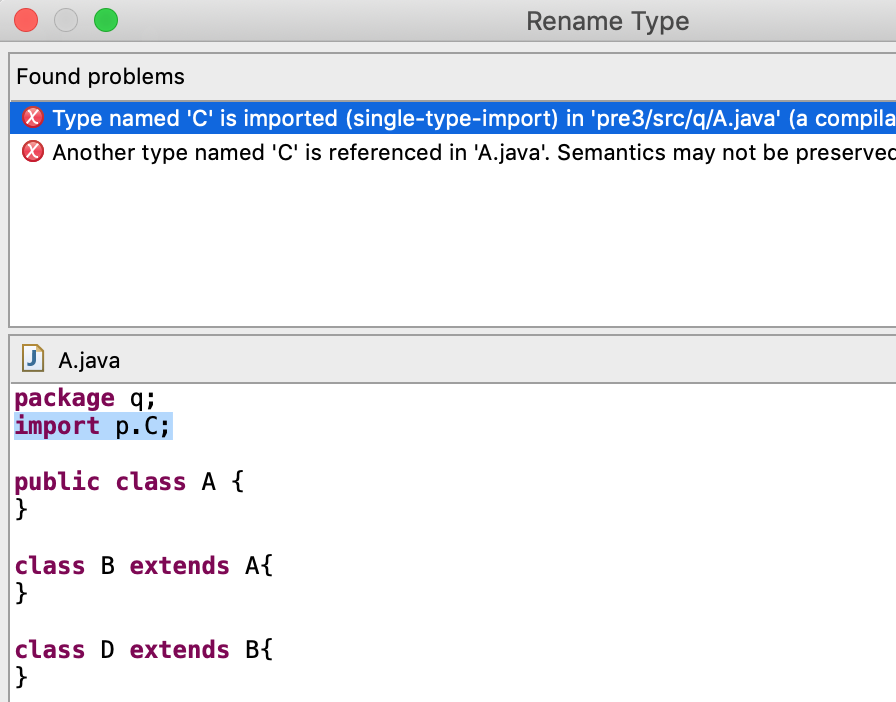
\includegraphics[width=85mm,scale=0.5]{precond3.png}}
\caption{Error produced after renaming the sub-class.}
\label{figure:fig8}
\end{figure}
